% !TeX program = xelatex
\documentclass[a4paper,12pt]{article}
% Личная преамбула и титульный лист; заполнить поля текущей работы.
\newcommand{\LabSubject}{Моделирование}
\newcommand{\LabWorkType}{УЧЕБНО-ИССЛЕДОВАТЕЛЬСКАЯ РАБОТА}
\newcommand{\LabNumber}{3}
\newcommand{\LabTopic}{Исследование СМО и СеМО}
\newcommand{\LabVariant}{41/3} % Пустое значение скрывает строку варианта.
\newcommand{\LabAuthor}{Михайлов Петр Сергеевич}
\newcommand{\LabGroup}{P3311}
\newcommand{\LabTeacher}{Вирта Виктория Владимировна}
\newcommand{\LabYear}{2026}

\usepackage{iftex}
\ifPDFTeX
  \usepackage[T2A]{fontenc}
  \usepackage[utf8]{inputenc}
  \usepackage[russian]{babel}
\else
  \usepackage{fontspec}
  \usepackage{polyglossia}
  \setdefaultlanguage{russian}
  \setotherlanguage{english}
  \IfFontExistsTF{Times New Roman}{%
    \setmainfont{Times New Roman}\newfontfamily\cyrillicfont{Times New Roman}}{%
    \IfFontExistsTF{NimbusRoman-Regular.otf}{%
      \setmainfont{NimbusRoman}[Extension=.otf,UprightFont=*-Regular,BoldFont=*-Bold,ItalicFont=*-Italic,BoldItalicFont=*-BoldItalic]
      \newfontfamily\cyrillicfont{NimbusRoman}[Extension=.otf,UprightFont=*-Regular,BoldFont=*-Bold,ItalicFont=*-Italic,BoldItalicFont=*-BoldItalic]
    }{\setmainfont{DejaVu Serif}\newfontfamily\cyrillicfont{DejaVu Serif}}}
  \setsansfont{Arial}
  \newfontfamily\cyrillicfontsf{Arial}
  \setmonofont{Consolas}
  \newfontfamily\cyrillicfonttt{Consolas}
\fi
\usepackage{amsmath,amssymb,amsfonts}
\usepackage{graphicx,geometry,listings,xcolor,hyperref,float,booktabs}
\usepackage{longtable,array,tabularx,caption}
\usepackage{tikz}
\usetikzlibrary{arrows.meta,fit,positioning}

\geometry{left=2cm,right=1.5cm,top=2cm,bottom=2cm}
\hypersetup{unicode=true,colorlinks=true,linkcolor=black,urlcolor=blue!60!black,
 pdftitle={\LabWorkType\space №\LabNumber. \LabTopic},pdfauthor={\LabAuthor}}
\captionsetup{font=small,labelsep=period}
\setlength{\parindent}{1.25cm}
\setlength{\parskip}{.2em}
\linespread{1.05}
\raggedbottom
\setcounter{tocdepth}{2}
\setlength{\emergencystretch}{2em}
\tolerance=3000
\lstdefinestyle{mypython}{language=Python,basicstyle=\ttfamily\scriptsize,
 keywordstyle=\color{blue!65!black}\bfseries,stringstyle=\color{red!65!black},
 commentstyle=\color{green!35!black},numbers=left,numberstyle=\tiny\color{gray},
 stepnumber=1,numbersep=7pt,showstringspaces=false,tabsize=4,frame=single,
 breaklines=true,breakatwhitespace=false,columns=fullflexible,keepspaces=true,
 xleftmargin=14pt,framexleftmargin=10pt,backgroundcolor=\color{gray!3}}
\lstset{style=mypython}
\usepackage{fancyvrb}
\makeatletter
\let\TableRows\@@input
\makeatother

\begin{document}
\begin{titlepage}
\centering
{\fontsize{11}{13}\selectfont\textbf{Министерство науки и высшего образования Российской Федерации}}\\
{\fontsize{7}{10}\selectfont ФЕДЕРАЛЬНОЕ ГОСУДАРСТВЕННОЕ АВТОНОМНОЕ ОБРАЗОВАТЕЛЬНОЕ УЧРЕЖДЕНИЕ ВЫСШЕГО ОБРАЗОВАНИЯ}\\
\vspace{.2cm}
{\fontsize{14}{17}\selectfont\textbf{«НАЦИОНАЛЬНЫЙ ИССЛЕДОВАТЕЛЬСКИЙ УНИВЕРСИТЕТ ИТМО»}}
\vspace{1cm}

{\fontsize{12}{14}\selectfont\textbf{Факультет программной инженерии и компьютерной техники}}
\vspace{1cm}

{\fontsize{12}{14}\selectfont\textbf{Дисциплина: \LabSubject}}
\vspace*{\fill}

{\fontsize{18}{22}\selectfont\textbf{\LabWorkType\ №\LabNumber}}\\
\vspace{.5cm}
{\fontsize{14}{17}\selectfont\textbf{по теме: «\LabTopic»}}
\vspace{1.5cm}

\ifx\LabVariant\empty\else{\fontsize{12}{14}\selectfont\textbf{Вариант: \LabVariant}}\fi
\vspace{1.5cm}
\begin{flushright}
\fontsize{12}{14}\selectfont
Выполнил:\\
\LabAuthor\\
Группа: \LabGroup\\[1em]
Преподаватель:\\
\LabTeacher
\end{flushright}
\vfill
{\fontsize{12}{14}\selectfont Санкт-Петербург, \LabYear}
\end{titlepage}
\setcounter{page}{2}
{\small\setlength{\parskip}{0pt}\tableofcontents}
\newpage

\section{Цель и постановка работы}

Цель работы — исследовать характеристики систем и сетей массового
обслуживания методом дискретно-событийного моделирования. В первой
части воспроизводится работа выбранной системы из УИР~2 и сравниваются
эффекты изменения поступления, обслуживания и структуры. Во второй
части исследуются замкнутая и разомкнутая сети топологии M3 по
варианту \(41/3\), определяется узкое место и сравниваются режимы
при одинаковом потоке на границе сети.

\section{Метод измерения}

Модельное время измеряется в секундах. В GPSS World транзакт
представляет заявку, а событие переводит её между узлами и фазами
обслуживания. Для сравнения учитываются продуктивные завершения,
потери, накопленное время пребывания и интегралы числа занятых
приборов и длины очереди. При оценке установившихся характеристик
после прогрева выполняется \texttt{RESET}: счётчики измерений
обнуляются при сохранении текущего состояния модели. Незавершённые
на границе измерения заявки учитываются при проверке баланса.

Все экспериментальные данные в работе получены в GPSS World.
Для контрольных прогонов сохранены стандартные отчёты, для
параметрических серий процедура PLUS выгружает измерения в CSV.
Скрипты Python читают эти файлы, рассчитывают сводные показатели
и строят графики. Аналитические модели используются для сверки.

При чтении стандартного отчёта загрузка приборов берётся из блока
\texttt{STORAGE}, средняя длина очереди — из \texttt{QUEUE}. Нулевое
ожидание учитывается в средних временах наравне с положительным.
Распределения ожидания и пребывания регистрируются посредством
\texttt{TABLE}, \texttt{QTABLE} и \texttt{TABULATE}.
Отношение числа завершений к времени наблюдения даёт
производительность \(X\), а произведение \(X\overline W\)
проверяет оценку средней длины очереди в стационарном режиме.

\section{Исследование системы массового обслуживания}
\label{sec:part1}

\subsection{Структура и проверка по УИР 2}

Исследуемая система состоит из двух параллельных ветвей.
В ветвь П1 направляется \(75\%\) заявок, в П2 — \(25\%\).
Перед П1 предусмотрено два места ожидания, перед П2 — одно.
При заполнении выбранной ветви заявка теряется. Среднее время
экспоненциального обслуживания в каждой ветви составляет \(5\) с.
Начальная контрольная точка соответствует интенсивности
\(\lambda=0{,}6\) заявки/с, принятой для системы 33 в УИР~2.

Суммарную ёмкость ветви в GPSS задаёт \texttt{STORAGE Cap},
ёмкость обслуживания — \texttt{STORAGE Srv}. Перед входом
\texttt{TEST} проверяет свободное место, блоки \texttt{QUEUE}
и \texttt{DEPART} регистрируют ожидание, а задержка в \texttt{ADVANCE}
соответствует обслуживанию. Заявка завершает обслуживание в
\texttt{Done}, отказ регистрируется в \texttt{Lost}.
Для расчёта \(\overline W\) и \(\overline T\) используются заявки,
закончившие обслуживание. Доля потерь определяется среди всех
завершившихся исходов, включая отказы. Значения по отдельным
приборам суммируются для загрузки и длины очереди.

\begin{table}[htbp]
  \centering
  \caption{Сверка исходной точки системы 33}
  \label{tab:p1-baseline}
  \begin{tabular}{@{}lrrr@{}}
  \toprule
  Характеристика & УИР~2 & GPSS World & Отклонение, \% \\
  \midrule
  Среднее число занятых приборов & 1,516814 & 1,518697 & $+0,12$\\
  Производительность, заявок/с & 0,303363 & 0,304447 & $+0,36$\\
  Вероятность потери & 0,494395 & 0,491417 & $-0,60$\\
  Средняя суммарная длина очереди & 1,656407 & 1,649222 & $-0,43$\\
  Среднее время ожидания, с & 5,460153 & 5,416749 & $-0,79$\\
  Среднее время пребывания, с & 10,460153 & 10,405015 & $-0,53$\\
  \bottomrule
  \end{tabular}
\end{table}

В измерительном интервале длиной \(200\,462{,}1\) с получено
\(61\,030\) завершений обслуживания и \(58\,970\) отказов.
Стандартный отчёт этого прогона показан на
рисунке~\ref{fig:gp-system-report}.
Наибольшее относительное отклонение в таблице~\ref{tab:p1-baseline}
составило \(0{,}79\%\). По формуле Литтла \(X\overline W=1{,}6491\),
что согласуется с интегральным средним числа заявок в очередях.
Отклонение от стационарного расчёта ожидаемо при конечной
длительности прогона.

\subsection{Эксперименты с потоком и обслуживанием}

Предложенная загрузка одного прибора в первой ветви задаётся как
\(\rho_1=0{,}75b/a\), где \(a\) — средний интервал на входе,
\(b\) — средняя длительность обслуживания, а \(0{,}75\) — вероятность
выбора ветви. Средний интервал \(a=11{,}5167\) с сохранён для всех
четырёх потоков. Значения \(\rho_1=0{,}50;\,0{,}75;\,0{,}95;\,0{,}99\)
получены подбором \(b\).

В GPSS World сравнивались простейший поток, циклическая трасса из
300 интервалов варианта 207, равномерный поток с интервалами из
\([0;2a]\) и гиперэкспоненциальная аппроксимация \(H_2\) из УИР~1.
Программа УИР~1 читала первую колонку исходного файла, содержащую
целые части интервалов. Для согласованности здесь повторно использована
эта последовательность со средним \(11{,}5167\) с и коэффициентом
вариации \(2{,}429\). Нулевые интервалы порождают заявки с одинаковым
временем поступления. Вес длинной фазы аппроксимации равен \(0{,}2319\).
Средние фаз \(44{,}32\) и \(1{,}61\) с масштабированы общим множителем,
чтобы среднее смеси совпало со средним трассы.

Параметрические серии выполнены средствами GPSS World. Для каждого
основного режима проведено три повтора по \(120\,000\) исходов после
\(10\,000\) исходов прогрева. В дополнительной серии изменения
\(a\) и \(b\) при простейшем потоке использован один прогон на режим.
Перед измерением команда \texttt{RESET}
сбрасывает статистику. Процедура PLUS записывает из модели значения
системных атрибутов и счётчики по завершении каждого прогона. В
таблицах приведены средние по повторам и суммарное число отказов.
Полосы на графиках показывают \(95\%\)-е интервалы Стьюдента по средним
отдельных повторов. Для трассы интервалы отражают разброс результатов
при разных реализациях маршрутизации и обслуживания на фиксированном
входе.

\begin{figure}[htbp]
 \centering
 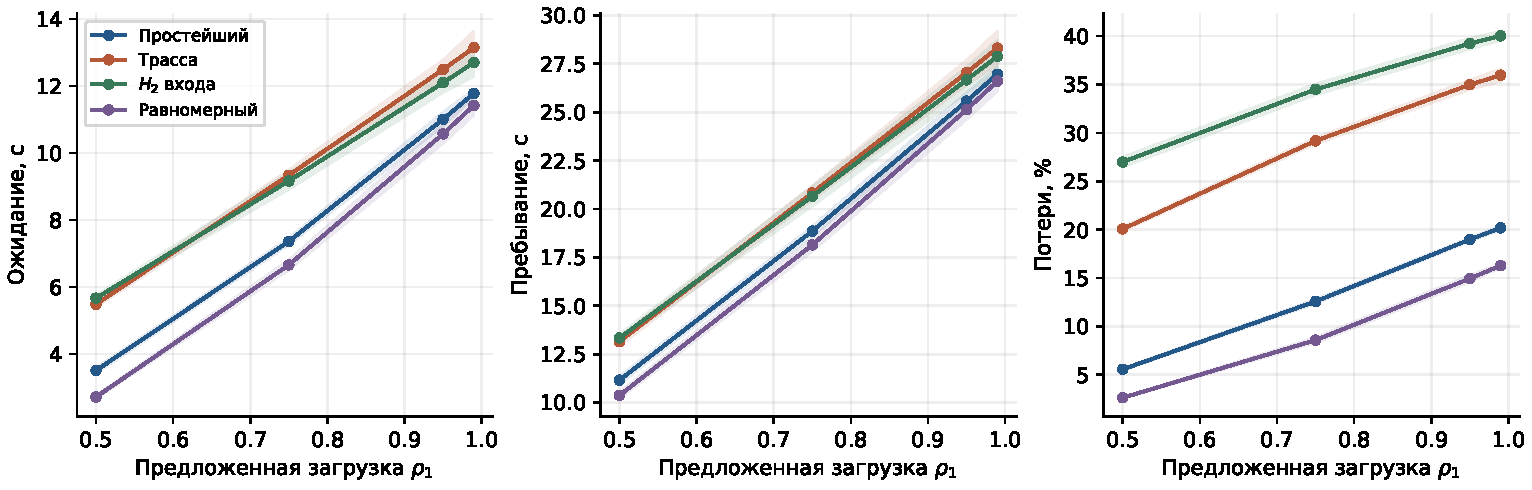
\includegraphics[width=\textwidth]{../out/part1/gpss/flows.pdf}
 \caption{Ожидание, пребывание и потери при смене входного потока}
 \label{fig:p1-flows}
\end{figure}

При простейшем потоке сравнивались экспоненциальный, эрланговский и
гиперэкспоненциальный законы обслуживания обоих приборов. Для \(E_2\)
длительность равна сумме двух экспоненциальных фаз со средним \(b/2\).
Для \(H_2\) с коэффициентом вариации 2 использованы веса
\(p=(1+\sqrt{3/5})/2\), \(1-p\) и средние фаз \(b/(2p)\),
\(b/[2(1-p)]\). Среднее обслуживания во всех случаях равно \(b\).

\begin{table}[htbp]
 \centering\small
 \caption{Смена входного потока или обслуживания при \(\rho_1=0{,}75\)}
 \label{tab:p1-flow-service}
 \begin{tabular}{@{}lrrrrrrr@{}}
 \toprule
 Вариант & Занято & Отказов & Потери, \% &
 \(\overline W\), с & \(\sigma_W\), с & \(\overline T\), с & \(\sigma_T\), с\\
 \midrule
 \TableRows ../out/part1/gpss/flow_service_rows.tex
 \bottomrule
 \end{tabular}
\end{table}

В первых четырёх строках таблицы~\ref{tab:p1-flow-service} фиксирован
экспоненциальный закон обслуживания. Последние две строки сравниваются
с первой при одинаковом простейшем потоке. Среднеквадратические
отклонения определены по заявкам, завершившим обслуживание.
Показатель «Занято» — среднее число занятых приборов в двух ветвях.
При замене входного потока доля потерь выросла с \(12{,}57\%\) до
\(29{,}17\%\) для трассы и до \(34{,}48\%\) для \(H_2\).
Короткие интервалы в этих потоках приводят к поступлению заявок
группами, и накопители быстрее заполняются. Равномерный поток
дал \(8{,}58\%\) потерь. При изменении обслуживания доля потерь
составила \(10{,}30\%\) для \(E_2\) и \(18{,}27\%\) для \(H_2\).
При \(\rho_1=0{,}99\) среднее ожидание простейшего режима равно
\(11{,}78\) с. Замена входа на \(H_2\) увеличила его до \(12{,}70\) с,
а замена обслуживания на \(H_2\) — до \(13{,}72\) с.

\begin{figure}[htbp]
 \centering
 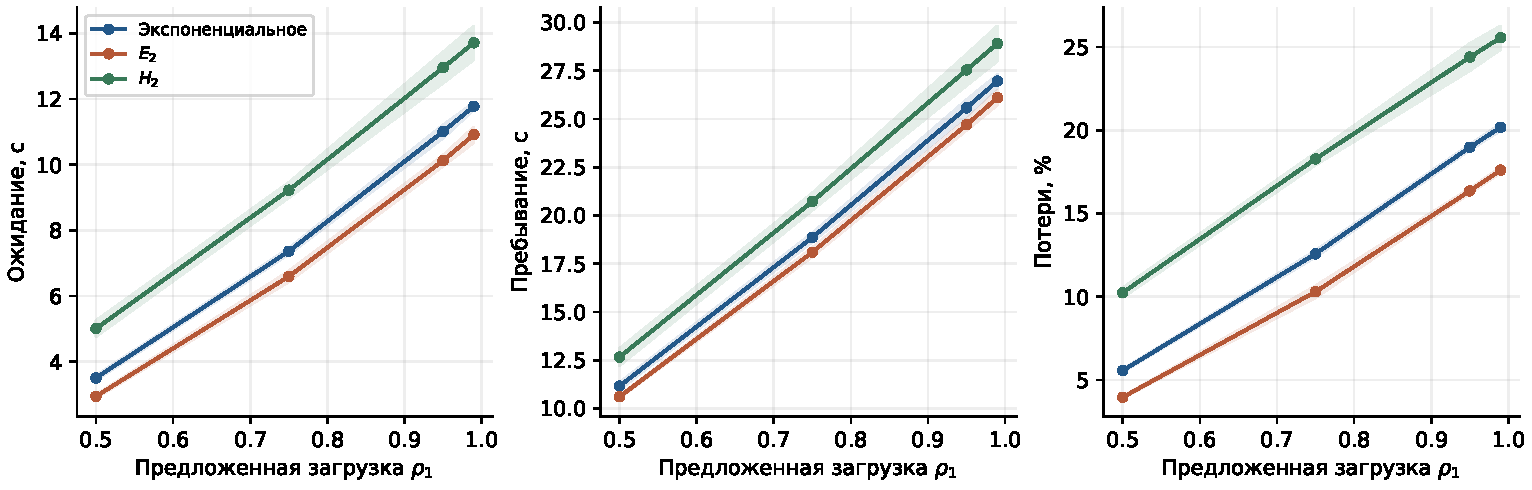
\includegraphics[width=\textwidth]{../out/part1/gpss/services.pdf}
 \caption{Характеристики СМО при смене закона обслуживания}
 \label{fig:p1-services}
\end{figure}

\subsection{Переходный режим}

Модель запускалась из пустого состояния. Накопленные оценки
\(\overline W\) и доли потерь после \(10\), \(50\), \(100\), \(200\),
\(300\), \(600\), \(1200\), \(2500\), \(5000\) и \(10\,000\) исходов
сравнивались со средними после прогрева. Точкой стабилизации принят
первый контрольный момент, начиная с которого все оставшиеся точки,
числом не меньше двух, укладываются в допуск. Для доли потерь допуск
составляет \(0{,}005\) по абсолютной величине, для ожидания — \(5\%\)
с нижней границей \(0{,}02\) с. В таблицах прочерк означает, что
на проверенной сетке критерий не выполнен. Выбор контрольных моментов
и начальное состояние влияют на полученную оценку.

\begin{table}[htbp]
 \centering\small
 \caption{Число исходов до стабилизации оценок для разных потоков}
 \label{tab:p1-transition}
 \begin{tabular}{@{}rrrr@{}}
 \toprule
 \(\rho_1\) & Простейший & Трасса & Аппроксимация \(H_2\)\\
 \midrule
 \TableRows ../out/part1/gpss/transition_rows.tex
 \bottomrule
 \end{tabular}
\end{table}

При простейшем потоке и \(\rho_1=0{,}75\) обе оценки вошли в допуск
с \(5000\) исходов. На той же загрузке трасса и \(H_2\) потребовали
бы более длинной серии контрольных точек. При \(\rho_1=0{,}99\)
критерий на выбранной сетке не выполнен ни для одного из трёх потоков.

В дополнительной серии с простейшим входом исследована загрузка
\(0{,}10;\,0{,}30;\,0{,}70;\,0{,}90\). Загрузка изменялась либо через
среднее обслуживание \(b\) при фиксированном интервале \(a=11{,}5167\) с,
либо через \(a\) при фиксированном \(b=5\) с.

\begin{table}[htbp]
 \centering\small
 \caption{Число исходов до стабилизации при двух способах задания нагрузки}
 \label{tab:p1-transition-load}
 \begin{tabular}{@{}rrr@{}}
 \toprule
 \(\rho_1\) & Фиксирован \(a\) & Фиксирован \(b\)\\
 \midrule
 \TableRows ../out/part1/gpss/transition_load_rows.tex
 \bottomrule
 \end{tabular}
\end{table}

\begin{figure}[htbp]
 \centering
 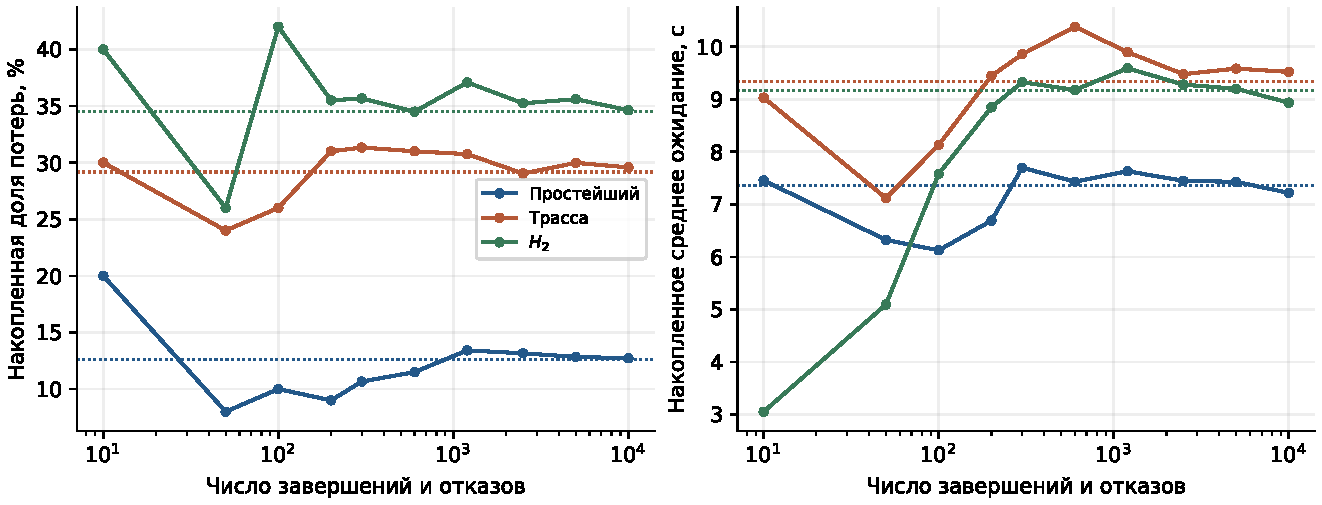
\includegraphics[width=.93\textwidth]{../out/part1/gpss/transition.pdf}
 \caption{Переход из пустого состояния при \(\rho_1=0{,}75\).
 Пунктиром показаны средние после прогрева}
 \label{fig:p1-transition}
\end{figure}

\subsection{Ёмкость накопителей и число приборов}

При простейшем входе и экспоненциальном обслуживании обеим ветвям
выделяли одинаковое число мест ожидания. Таблица~\ref{tab:p1-buffers}
показывает исходные режимы, результаты с восьмью местами на ветвь
и первые из проверенных ёмкостей, при которых во всех повторах
отсутствовали отказы за измерительный интервал, вместе с ближайшими
меньшими ёмкостями на сетке. По
рисунку~\ref{fig:p1-buffers} виден обмен между длиной ожидания и
долей потерь. При \(\rho_1=0{,}90\) восемь мест ожидания на ветвь
снизили потери с \(41{,}20\%\) до \(4{,}49\%\), при этом среднее
ожидание выросло с нуля до \(35{,}00\) с. Первые из проверенных
ёмкостей без отказов составили \(32\) и \(128\) мест на ветвь при
\(\rho_1=0{,}50\) и \(0{,}90\) соответственно. При \(256\) местах
максимальные длины очереди среди ветвей и повторов равны \(18\) и
\(99\). Оценка достаточной ёмкости зависит от длительности
наблюдения и генераторов. При
неограниченной длительности обслуживания и положительной
интенсивности потока любой конечный накопитель может переполниться.

\begin{table}[htbp]
 \centering\small
 \caption{Потери и времена при выбранных ёмкостях накопителей}
 \label{tab:p1-buffers}
 \begin{tabular}{@{}rrrrrr@{}}
 \toprule
 \(\rho_1\) & Мест на ветвь & Отказов & Потери, \% &
 \(\overline W\), с & \(\overline T\), с\\
 \midrule
 \TableRows ../out/part1/gpss/buffers_rows.tex
 \bottomrule
 \end{tabular}
\end{table}

\begin{figure}[htbp]
 \centering
 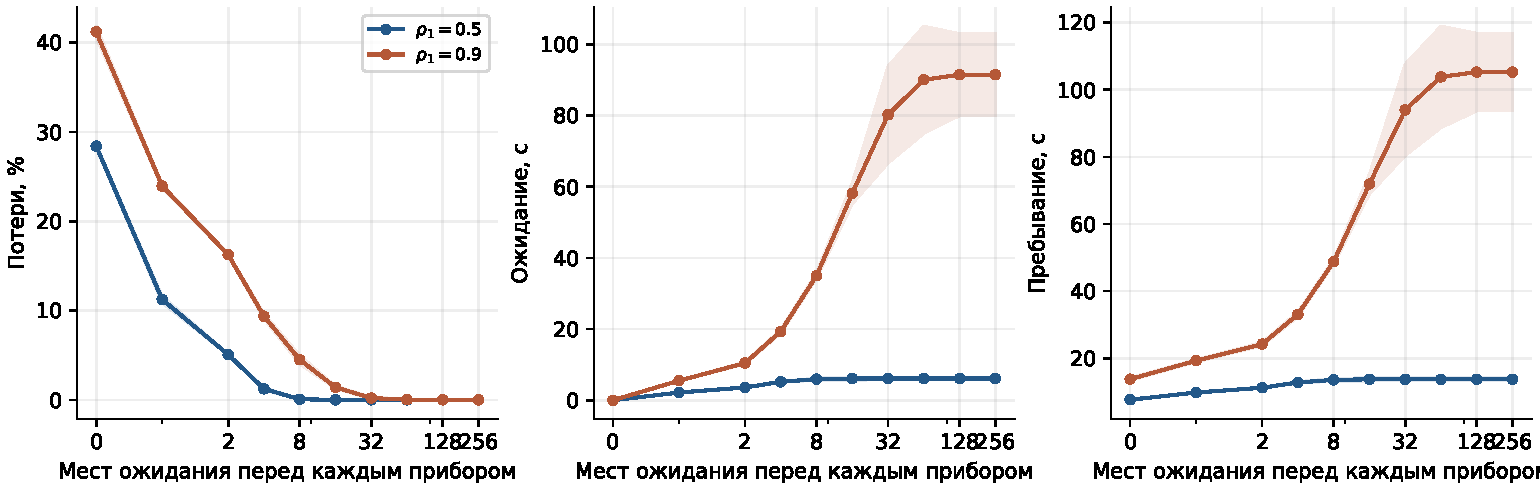
\includegraphics[width=\textwidth]{../out/part1/gpss/buffers.pdf}
 \caption{Потери и задержки при изменении ёмкости накопителей}
 \label{fig:p1-buffers}
\end{figure}

Для одного прибора весь поток направляется в одну очередь с двумя
местами ожидания. Исходная схема с двумя приборами сохраняет
разветвление \(0{,}75/0{,}25\). Третий прибор добавляется в первую
ветвь и обслуживает её общую очередь. При сравнении сохраняется
интенсивность входа, а среднее время обслуживания либо оставляется
тем же, либо подбирается под одинаковую предложенную загрузку
одного прибора первой ветви. Если в первой ветви \(c_1\) приборов
и вероятность выбора этой ветви равна \(p_1\), загрузка рассчитывается
как \(p_1 b/(c_1 a)\).

\begin{table}[htbp]
 \centering\small
 \caption{Число приборов при исходной загрузке \(\rho_1=0{,}75\)}
 \label{tab:p1-servers}
 \begin{tabular}{@{}lrrrrr@{}}
 \toprule
 Фиксируется & Приборов & \(\rho_1\) & \(b\), с &
 \(\overline W\), с & \(\overline T\), с\\
 \midrule
 \TableRows ../out/part1/gpss/servers_rows.tex
 \bottomrule
 \end{tabular}
\end{table}

При одинаковом времени обслуживания увеличение числа приборов
с одного до трёх снизило среднее ожидание с \(11{,}43\) до \(1{,}55\) с,
а среднее пребывание — с \(22{,}89\) до \(13{,}03\) с. В серии
с одинаковой загрузкой пребывание при трёх приборах выросло до
\(30{,}30\) с. Время обслуживания в этом опыте увеличивалось
вместе с числом приборов и непосредственно входило во время пребывания.

\begin{figure}[htbp]
 \centering
 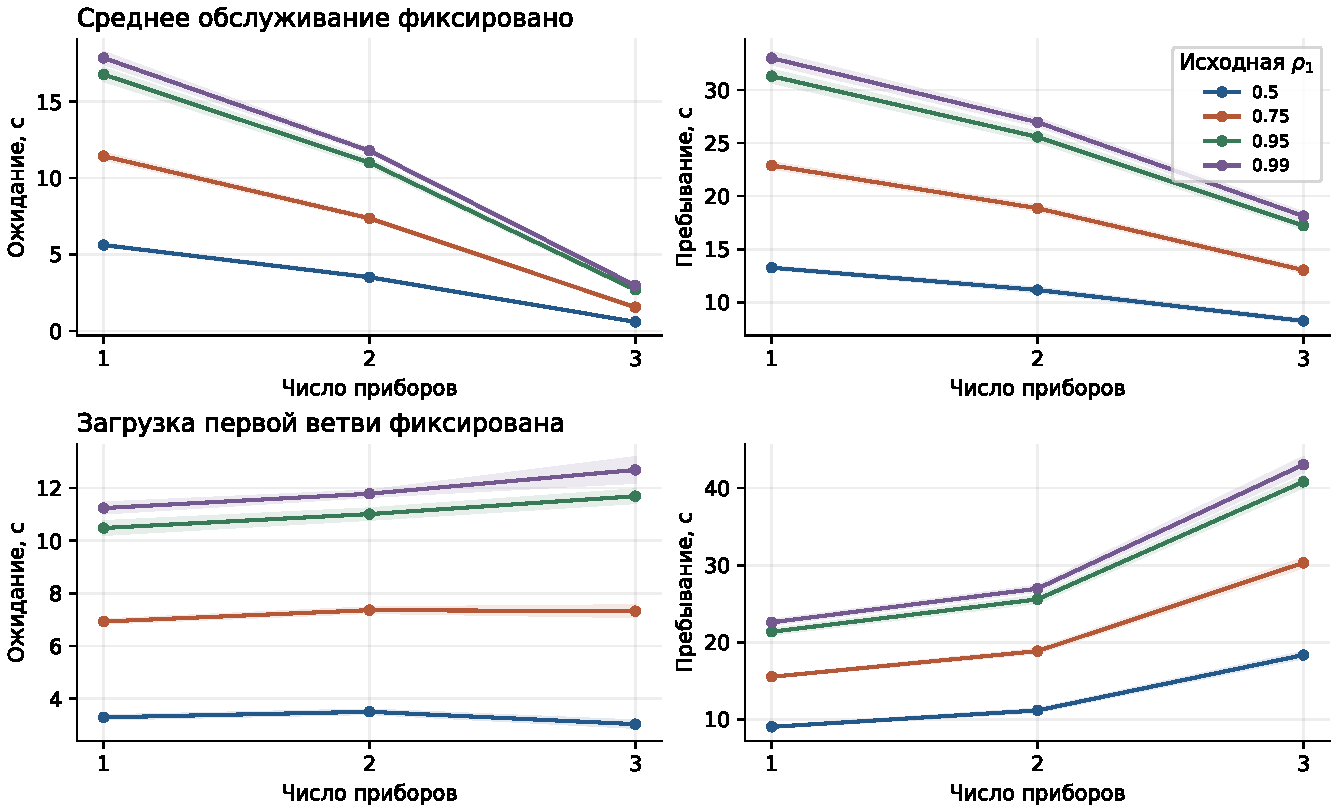
\includegraphics[width=.92\textwidth]{../out/part1/gpss/servers.pdf}
 \caption{Влияние числа приборов. В верхнем ряду фиксировано
 среднее обслуживание, в нижнем — загрузка первой ветви}
 \label{fig:p1-servers}
\end{figure}

\subsection{Проверка по формулам и форма распределений}

В контрольных прогонах использовалась одноканальная СМО с
простейшим потоком и накопителем на \(256\) мест. Для среднего
ожидания и пребывания при \(\rho=\lambda b<1\) использована
формула Поллачека — Хинчина
\[
 \overline W=\frac{\lambda\,\mathrm E[S^2]}{2(1-\rho)}
             =\frac{\rho b(1+c_s^2)}{2(1-\rho)},\qquad
 \overline T=\overline W+b.
\]
Здесь \(S\) — время обслуживания, \(c_s\) — его коэффициент
вариации. Для \(M/M/1\) принято \(c_s=1\), для \(M/G/1\) с
\(H_2\)-обслуживанием \(c_s=2\). В таблице~\ref{tab:p1-controls}
относительное отклонение \(\Delta_W\) рассчитано от теоретического
ожидания. В четырёх контрольных режимах потерь не наблюдалось.
Расхождение среднего ожидания с аналитическим расчётом не превысило
\(1{,}64\%\) для \(M/M/1\) и \(1{,}45\%\) для \(M/G/1\).

\begin{table}[htbp]
 \centering\small
 \caption{Сравнение одноканальных контролей с аналитическим расчётом}
 \label{tab:p1-controls}
 \begin{tabular}{@{}lrrrrrrr@{}}
 \toprule
 Модель & \(\rho\) &
 \(W_\text{расч}\), с & \(W_\text{GPSS}\), с & \(\Delta_W\), \% &
 \(T_\text{расч}\), с & \(T_\text{GPSS}\), с & Отказов\\
 \midrule
 \TableRows ../out/part1/gpss/controls_rows.tex
 \bottomrule
 \end{tabular}
\end{table}

\begin{table}[htbp]
 \centering\small
 \caption{Коэффициенты вариации задержек при \(\rho_1=0{,}75\)}
 \label{tab:p1-variation}
 \begin{tabular}{@{}lrrrr@{}}
 \toprule
 Поток & \(P(W=0)\), \% & \(c_W\) & \(c_{W\mid W>0}\) & \(c_T\)\\
 \midrule
 \TableRows ../out/part1/gpss/variation_rows.tex
 \bottomrule
 \end{tabular}
\end{table}

Ожидание имеет массу в нуле и положительную составляющую. Для
положительных задержек коэффициент вариации в четырёх опытах
лежит в пределах \(0{,}90\)–\(0{,}92\), а для пребывания —
\(0{,}86\)–\(0{,}92\). По относительному разбросу эти величины
близки к экспоненциальным. Для идентификации закона нужны данные
о форме распределения, в частности частоты из таблиц GPSS World.

\section{Исследование сетей массового обслуживания}
\label{sec:part2}

\subsection{Исходные данные и граф модели M3}

В сети варианта \(41/3\) четыре узла с числом приборов
\(c=(3,2,1,1)\) и средним временем обслуживания
\(b=(4;2{,}5;14;5)\) с. Ёмкость очередей не ограничена. Заявки
в каждом узле обслуживаются в порядке поступления. Переходы между
узлами мгновенны.
После обслуживания в У1 заявка с равной вероятностью \(0{,}25\)
переходит в У2, У3, У4 или в точку 0. После периферийного узла она
всегда возвращается в У1. В замкнутой сети точка 0 отмечает конец
цикла и мгновенный вход в следующий цикл. В разомкнутой сети она
означает внешний источник на входе и сток на выходе.

\begin{figure}[htbp]
  \centering
  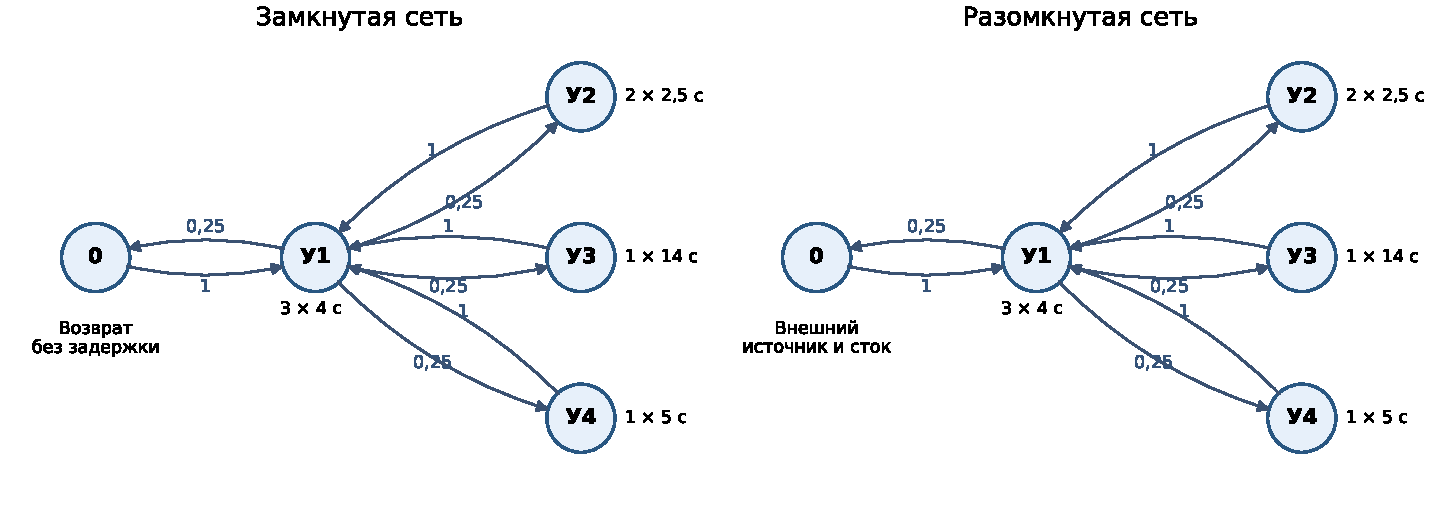
\includegraphics[width=\textwidth]{../out/part2/topology.pdf}
  \caption{Графы замкнутой и разомкнутой СеМО. В узлах указаны
  число приборов и средняя длительность обслуживания.}
  \label{fig:p2-network}
\end{figure}

При нормировке на выход одной заявки через точку 0 уравнения потоков
имеют вид
\[
  v_0=1,\qquad v_1=1+v_2+v_3+v_4,\qquad
  v_2=v_3=v_4=0{,}25v_1.
\]
Поэтому коэффициенты передач равны \(v=(4,1,1,1)\).
За цикл заявка в среднем проходит У1 четыре раза и по одному разу
посещает каждый периферийный узел. Суммарная потребность цикла в
обслуживании составляет \(\sum_i v_i b_i=37{,}5\) с. Потребность в
расчёте на один прибор составляет
\[
  \left(\frac{v_i b_i}{c_i}\right)_{i=1}^4
  = \left(\frac{16}{3};1{,}25;14;5\right)\ \text{с}.
\]
У3 ограничивает пропускную способность сети
\(X_{\max}=\min_i c_i/(v_i b_i)=1/14=0{,}071429\) заявки/с.
Для устойчивости разомкнутой сети нужно \(\lambda<X_{\max}\).
При \(\lambda=X_{\max}\) загрузка У3 достигает единицы, и конечное
стационарное среднее очереди к этому узлу отсутствует.

\subsection{GPSS-модель и план эксперимента}

Каждый узел использует последовательность блоков \texttt{QUEUE},
\texttt{ENTER}, \texttt{DEPART}, \texttt{ADVANCE}, \texttt{LEAVE}.
Ёмкость \texttt{STORAGE} равна числу одинаковых параллельных приборов.
После \texttt{MARK~2} значение \texttt{MP2} измеряет время с входа
в текущий узел. При входе в прибор это ожидание прибавляется к
параметру заявки, а после обслуживания по \texttt{MP2} измеряется
полное время посещения. В точке 0 \texttt{TABULATE} записывает
накопленное ожидание и длительность цикла либо пребывания заявки.
Маршрут из У1 выбирается по равномерному случайному числу из
1000 значений. Каждому из четырёх маршрутов соответствуют
250 значений. Из остальных узлов заявки возвращаются в У1.

В замкнутом варианте на старте создаётся \(M\) транзактов. В
разомкнутом варианте внешние заявки поступают через интервалы со
средним \(1/\lambda\), распределённые экспоненциально или заданные
постоянными. После прохождения У1 и выбора маршрута в точку 0
транзакт возвращается в замкнутую сеть или покидает разомкнутую.
Во всех опытах меняется одно указанное условие при сохранении
параметров базовой модели. Для исследования разброса времени
обслуживания меняется закон только в У2 при прежнем среднем
\(b_2=2{,}5\) с. Использованы экспоненциальное распределение,
\(E_2\) как сумма двух независимых экспоненциальных величин со
средним \(1{,}25\) с и гиперэкспоненциальное \(H_2\) с
коэффициентом вариации 2. В последнем случае выбирается одна из
двух экспоненциальных компонент с параметрами
\[
  p=\frac{1-\sqrt{3/5}}{2},\quad
  b_{21}=\frac{2{,}5}{2p},\quad b_{22}=\frac{2{,}5}{2(1-p)}.
\]
Обе компоненты вносят одинаковый вклад в общее среднее. Так
изменение длительности ожидания можно связать с разбросом
обслуживания и взаимодействием узлов.

Производительность \(X\) считали по числу завершённых циклов
или выходов за единицу времени. Чтобы сопоставить нагрузки, задавали
\(\lambda=X\) при одном и том же законе обслуживания в У2.
При фиксированном \(M\) проверили два способа разгрузить У3.
Среднее время обслуживания сокращали с 14 до 5 с или увеличивали
число приборов с одного до трёх. В обоих случаях наибольшая
потребность на прибор приходится на У1.

\subsection{Аналитическая проверка экспоненциальных моделей}

Для замкнутой сети с экспоненциальным обслуживанием рассчитаны
точные стационарные показатели. При состоянии
\(n=(n_1,\ldots,n_4)\), \(\sum_i n_i=M\), ненормированный вес равен
\[
  w(n)=\prod_{i=1}^4
      \frac{(v_i b_i)^{n_i}}{\prod_{j=1}^{n_i}\min(j,c_i)},\qquad
  G(M)=\sum_{\sum_i n_i=M}w(n),\qquad X(M)=\frac{G(M-1)}{G(M)}.
\]
Пустое произведение равно единице. Из сохранения популяции по
формуле Литтла среднее время цикла равно \(M/X(M)\). Для
разомкнутой экспоненциальной сети интенсивность в У\(i\) равна
\(\lambda v_i\), и ожидание в нём рассчитано по формуле Эрланга C
для \(M/M/c_i\). Сетевое ожидание — сумма узловых с весами \(v_i\).

Критическим считали наименьшее \(M\), при котором отставание
от предельной производительности \(1-X(M)/X_{\max}\) не превышает \(2\%\).
При \(M=5\) расчёт даёт \(X=0{,}068601\) заявки/с
(\(3{,}96\%\) до предела), при \(M=6\) — \(0{,}070167\) заявки/с
(\(1{,}77\%\)). Таким образом, \(M^*=6\).
Рост \(M\) сначала сокращает простой У3, поэтому растёт
производительность. Затем У3 почти всё время занят, новые заявки
в основном увеличивают очередь. При почти постоянном \(X\) среднее
время цикла \(M/X\) продолжает расти почти линейно. В разомкнутой
сети механизм иной: при приближении \(\lambda\) к \(1/14\) в У3
время ожидания растёт примерно как \(1/(1/14-\lambda)\), поскольку
внешний источник не ограничивает суммарное число заявок.

\subsection{Замкнутая сеть и устранение узкого места}

В основной серии GPSS World для каждой из 37 конфигураций сделали
по три прогона. Модель прогревали \(25\,000\) с, затем собирали
данные \(250\,000\) с. Начальные состояния генераторов меняли
между повторами. При сравнении конфигураций в одном повторе
их сохраняли, чтобы уменьшить вклад случайного разброса. На графиках
отрезки показывают одно стандартное отклонение по прогонам.

При \(M=5\) среднее измеренное \(X=0{,}069228\) заявки/с
на \(3{,}08\%\) ниже предела, при \(M=6\) значение
\(X=0{,}070864\) заявки/с находится на расстоянии \(0{,}79\%\)
от предела. Первый переход через уровень \(98\%\) предельной
производительности подтверждает \(M^*=6\). В этой точке среднее
время цикла составило \(84{,}66\) с, а по формуле Литтла с
измеренным \(X\) получается \(M/X=84{,}67\) с. Точный расчёт
для этой точки даёт \(X=0{,}070167\) заявки/с. Различие
с измерением составило \(0{,}99\%\). При \(M\geq7\) часть
конечных оценок \(X\) немного выше \(1/14\). Предельная
пропускная способность относится к установившемуся среднему,
тогда как в конкретной реализации длительности обслуживания
случайны.

\begin{figure}[htbp]
 \centering
 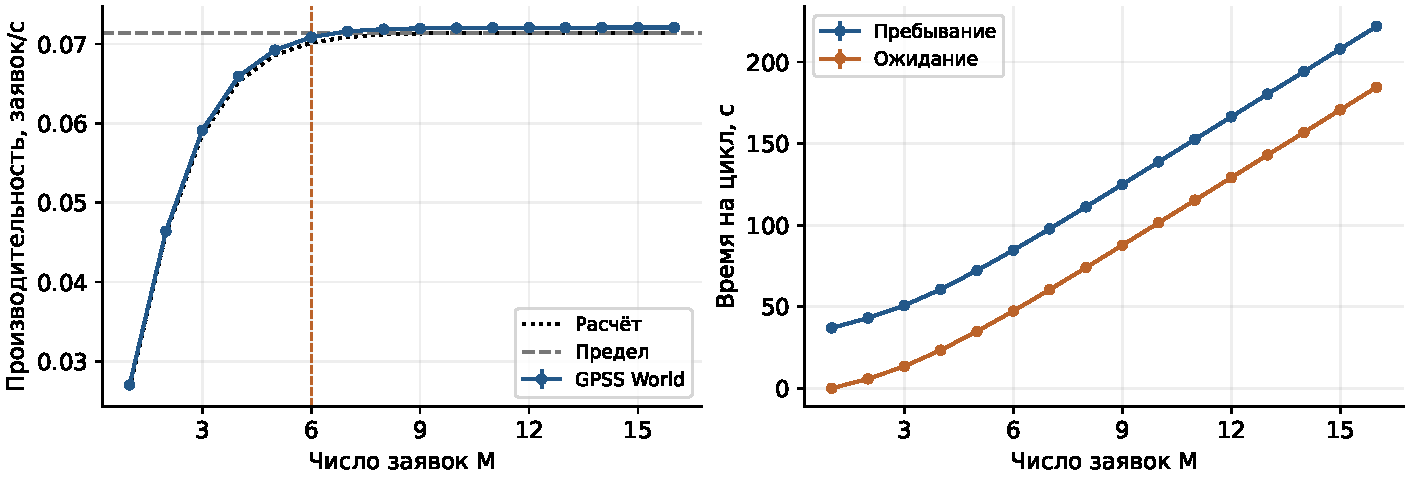
\includegraphics[width=\textwidth]{../out/part2/gpss/closed_scaling.pdf}
 \caption{Производительность и длительность цикла замкнутой сети}
 \label{fig:p2-scaling}
\end{figure}

\begin{table}[htbp]
 \centering
 \caption{Эффект устранения узкого места в замкнутой сети при \(M=6\)}
 \label{tab:p2-bottleneck}
 \begin{tabular}{@{}lrrrr@{}}
 \toprule
 Конфигурация & \(X\), заявок/с & \(\overline W\), с & \(\overline T\), с & \(\rho_3\) \\
 \midrule
 Исходная         & 0,07086 & 47,37 & 84,66 & 0,982\\
 \(b_3=5\) с      & 0,13646 & 15,55 & 43,96 & 0,677\\
 \(c_3=3\)        & 0,12952 &  8,98 & 46,32 & 0,599\\
 \bottomrule
 \end{tabular}
\end{table}

При уменьшении \(b_3\) или увеличении \(c_3\) производительность
выросла соответственно в \(1{,}93\) и \(1{,}83\) раза. Три
прибора У3 сильнее сокращают ожидание, но время пребывания
чуть выше, чем при \(b_3=5\) с. В конфигурации с тремя
приборами длительность обслуживания в У3 остаётся равной
\(14\) с. Оба изменения переносят ограничение в У1.
Предельная производительность становится равной
\(3/16=0{,}1875\) заявки/с.

При \(M=6\) смена закона в У2 почти не изменила среднее время
пребывания в сети. Оно составило \(84{,}66\) с для
экспоненциального закона, \(84{,}66\) с для \(E_2\) и
\(84{,}67\) с для \(H_2\). Стандартное отклонение по прогонам
намного больше разницы между этими средними. В самом У2 среднее
ожидание на тех же прогонах составляет \(0{,}0177\),
\(0{,}0159\) и \(0{,}0262\) с. У2 имеет два прибора
и низкую загрузку. Основное ожидание приходится на У3,
поэтому влияние формы распределения обслуживания лучше
видно в узловой статистике.

\begin{figure}[htbp]
 \centering
 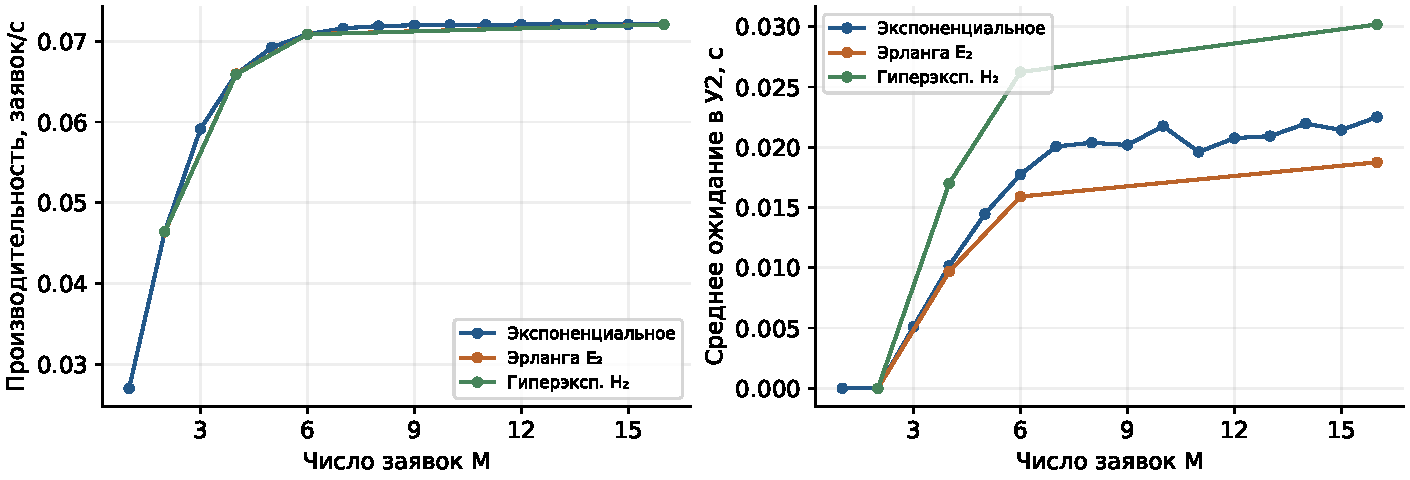
\includegraphics[width=\textwidth]{../out/part2/gpss/closed_service.pdf}
 \caption{Влияние закона обслуживания У2 при разных популяциях}
 \label{fig:p2-closed-service}
\end{figure}

\subsection{Разомкнутая сеть}

При простейшем внешнем потоке и экспоненциальном обслуживании
производительность в устойчивом режиме равна интенсивности
входа. При росте заданной нагрузки У3 с \(0{,}80\) до
\(0{,}95\) среднее пребывание увеличилось с \(90{,}37\) до
\(224{,}89\) с. Измеренная загрузка У3 выросла с \(0{,}777\)
до \(0{,}925\), а среднее число ожидающих в его очереди —
с \(2{,}86\) до \(12{,}38\). В верхней точке межпрогонное
стандартное отклонение времени пребывания составило
\(24{,}71\) с, оценка производительности — \(0{,}066915\)
заявки/с при заданных \(0{,}067857\) заявки/с. Точный расчёт при номинальной нагрузке
\(0{,}95\) даёт \(307{,}01\) с. В этой области среднее
ожидание чувствительно к изменению фактической загрузки,
поэтому даже небольшое отклонение входной производительности
и длительности обслуживания в отдельной реализации заметно
сказывается на оценке задержки.

\begin{figure}[htbp]
 \centering
 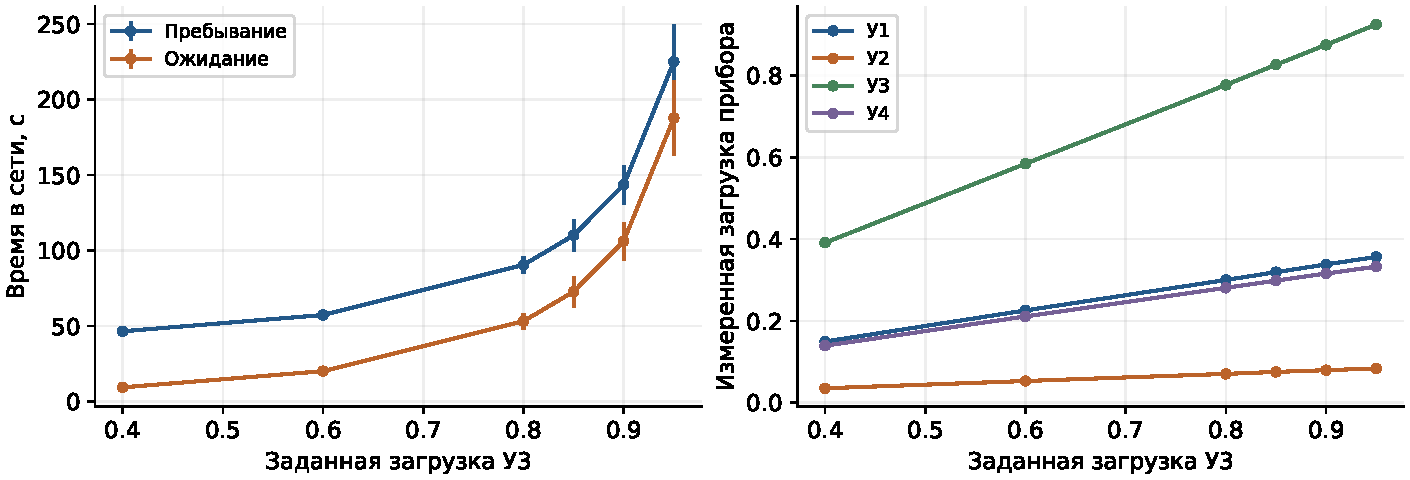
\includegraphics[width=\textwidth]{../out/part2/gpss/open_load.pdf}
 \caption{Задержки и загрузка узлов разомкнутой сети}
 \label{fig:p2-open}
\end{figure}

Законы обслуживания также сравнили при одной и той же заданной
нагрузке \(\rho_3=0{,}90\). При простейшем внешнем
потоке среднее ожидание в У2 составляет \(0{,}0173\),
\(0{,}0126\) и \(0{,}0263\) с для экспоненциального
обслуживания, \(E_2\) и \(H_2\). Коэффициент вариации
времени пребывания в У2 соответственно равен \(0{,}99\),
\(0{,}70\) и \(1{,}97\). С детерминированным внешним
потоком среднее ожидание в У2 составило \(0{,}0120\), \(0{,}0099\) и
\(0{,}0184\) с. При заданной интенсивности форма закона У2
практически не меняет загрузку У3. Замена внешнего потока
снизила среднее сетевое пребывание с \(143{,}42\) до
\(124{,}19\) с при экспоненциальном обслуживании. Изменение
сопоставимо с разбросом между повторами, поэтому вывод
относится к наблюдаемому эффекту в этих опытах.
Коэффициент вариации сетевого пребывания при простейшем
потоке практически одинаков для всех трёх законов У2
(\(1{,}85\)–\(1{,}87\)), с регулярным потоком он лежит
в диапазоне \(1{,}80\)–\(1{,}82\). Коэффициент вариации
сетевого ожидания для этих же конфигураций составлял
\(2{,}25\)–\(2{,}29\). Задержки в У3 определяют общий
разброс сильнее, чем изменение формы обслуживания в У2.

\subsection{Сопоставление сетей при равном потоке}

Для каждого закона обслуживания У2 измерили среднее \(X\)
замкнутой сети при \(M=6\) и задали такую же интенсивность входа
в разомкнутой модели. Заданная загрузка У3 получилась около
\(0{,}992\), поэтому прогрев увеличили до \(100\,000\) с,
а время наблюдения — до \(800\,000\) с. Для разомкнутой сети
проверили шесть конфигураций, по три прогона на каждую.
В таблице~\ref{tab:p2-matched} после знака \(\pm\) указаны
стандартные отклонения по повторам. Журнал завершённой серии
показан на рисунке~\ref{fig:gp-network-campaign}.

\begin{table}[htbp]
 \centering
 \caption{Среднее пребывание при совпадении интенсивности входа РСеМО
 и производительности ЗСеМО для каждого закона У2}
 \label{tab:p2-matched}
 \begin{tabular}{@{}lrrrr@{}}
 \toprule
 Закон У2 & \(\lambda\), заявок/с & ЗСеМО, с &
 \multicolumn{2}{c@{}}{РСеМО, с} \\
 \cmidrule(l){4-5}
 & & & Простейший поток & Регулярный поток \\
 \midrule
 Экспоненциальный & 0,070864 & 84,66 & \(1061{,}52\pm629{,}38\) & \(721{,}65\pm260{,}00\) \\
 \(E_2\)          & 0,070867 & 84,66 & \(1063{,}48\pm631{,}17\) & \(723{,}41\pm261{,}19\) \\
 \(H_2\)          & 0,070847 & 84,67 & \(1048{,}23\pm618{,}85\) & \(711{,}04\pm252{,}90\) \\
 \bottomrule
 \end{tabular}
\end{table}

Для экспоненциальной пары измеренная производительность
открытой сети с простейшим потоком составила \(0{,}070763\)
заявки/с, что на \(0{,}14\%\) ниже заданной интенсивности.
В разомкнутой сети среднее время пребывания больше
из-за накопления очереди в У3 при загрузке, близкой
к единице. В замкнутой сети общее число заявок
ограничено шестью. Регулярный внешний поток даёт
меньшие средние во всех трёх парах. При этом разброс
сетевого времени между прогонами велик, поэтому малые
различия между законами обслуживания У2 интерпретируются
по узловой статистике и по опытам при меньшей нагрузке.
Точный экспоненциальный расчёт при \(\lambda=0{,}070864\)
даёт \(1798{,}58\) с. Отличие от имитационной оценки
указывает на высокую неопределённость численного сравнения
вблизи границы устойчивости.

\begin{figure}[htbp]
 \centering
 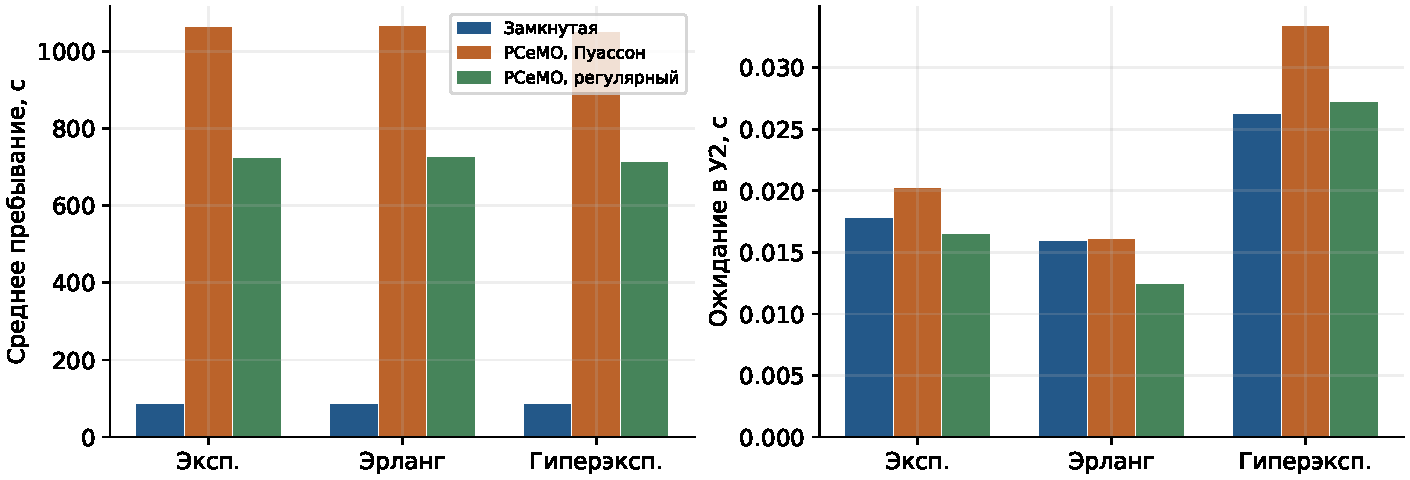
\includegraphics[width=\textwidth]{../out/part2/gpss/matched_service.pdf}
 \caption{Сравнение сетевого пребывания и ожидания в У2 при равном потоке}
 \label{fig:p2-match}
\end{figure}

\subsection{Распределения времени}

Для гистограмм на рисунке~\ref{fig:p2-native-hist} взяли частоты
из отчёта GPSS World по контрольному прогону замкнутой сети
при \(M=6\) (рисунок~\ref{fig:gp-network-report}).
За \(200\,000\) с измерения завершился
\(14\,221\) цикл. Среднее время цикла равно \(84{,}38\) с,
коэффициент вариации — \(1{,}30\). Аппроксимация \(H_2\)
по первым двум моментам даёт вероятность длинной компоненты
\(0{,}246\) и средние компонент \(171{,}56\) и \(55{,}94\) с.
На гистограмме много коротких циклов и заметен длинный правый
хвост. Параметры приближения подобраны по двум моментам, а саму
форму распределения показывает гистограмма.

Для пребывания в У2 коэффициент вариации \(0{,}98\)
близок к единице, что согласуется с экспоненциальной
аппроксимацией при базовом законе обслуживания. Ожидание
равно нулю в \(37{,}5\%\) циклов и \(98{,}6\%\) посещений
У2. Для аппроксимации ожидания эту вероятность выделяют
отдельно, а положительную часть описывают непрерывным
распределением. В разомкнутой сети высокие коэффициенты
вариации сетевого ожидания показывают, что существенная
часть разброса теряется при сравнении средних.

\begin{figure}[htbp]
 \centering
 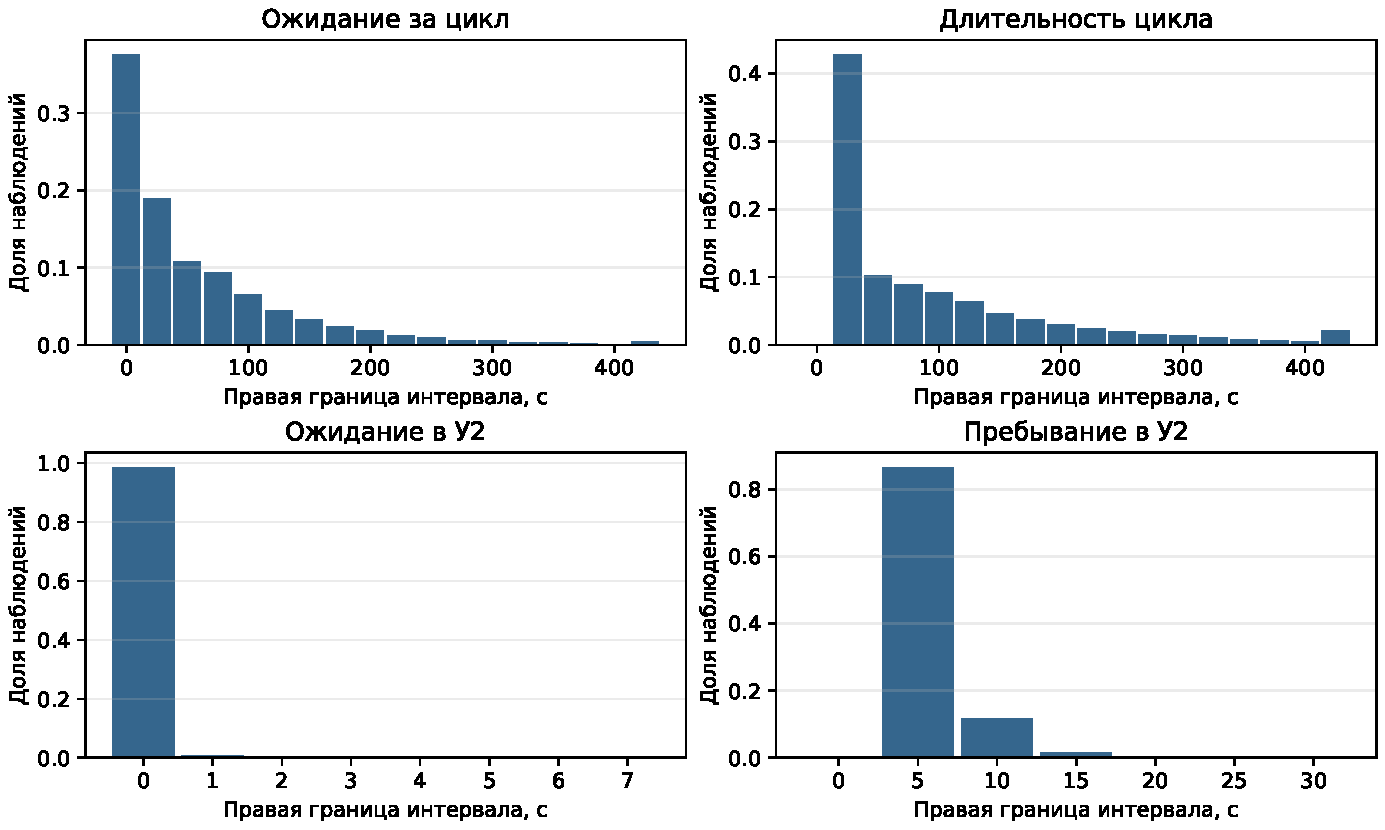
\includegraphics[width=.96\textwidth]{../out/part2/gpss_closed_histograms.pdf}
 \caption{Гистограммы сетевых и узловых времён из GPSS World.
 Замкнутая сеть, \(M=6\), экспоненциальное обслуживание}
 \label{fig:p2-native-hist}
\end{figure}

Для разомкнутой экспоненциальной сети при заданной
\(\rho_3=0{,}90\) контрольный прогон дал \(12\,634\) завершённых
заявки за \(200\,000\) с измерения. Среднее пребывание равно
\(120{,}06\) с при коэффициенте вариации \(1{,}62\).
Двухкомпонентная аппроксимация по моментам даёт вероятность
длинной компоненты \(0{,}166\) и средние \(362{,}23\)
и \(71{,}96\) с. В У2 коэффициент вариации пребывания
практически такой же, как в замкнутой сети (\(0{,}99\)).
Сетевое ожидание равно нулю в \(41{,}8\%\) наблюдений.
При этом длинные ожидания дают среднее \(83{,}23\) с.
Нулевая масса и длинный хвост видны одновременно на
сетевой гистограмме (рисунок~\ref{fig:p2-open-hist}).

\begin{figure}[htbp]
 \centering
 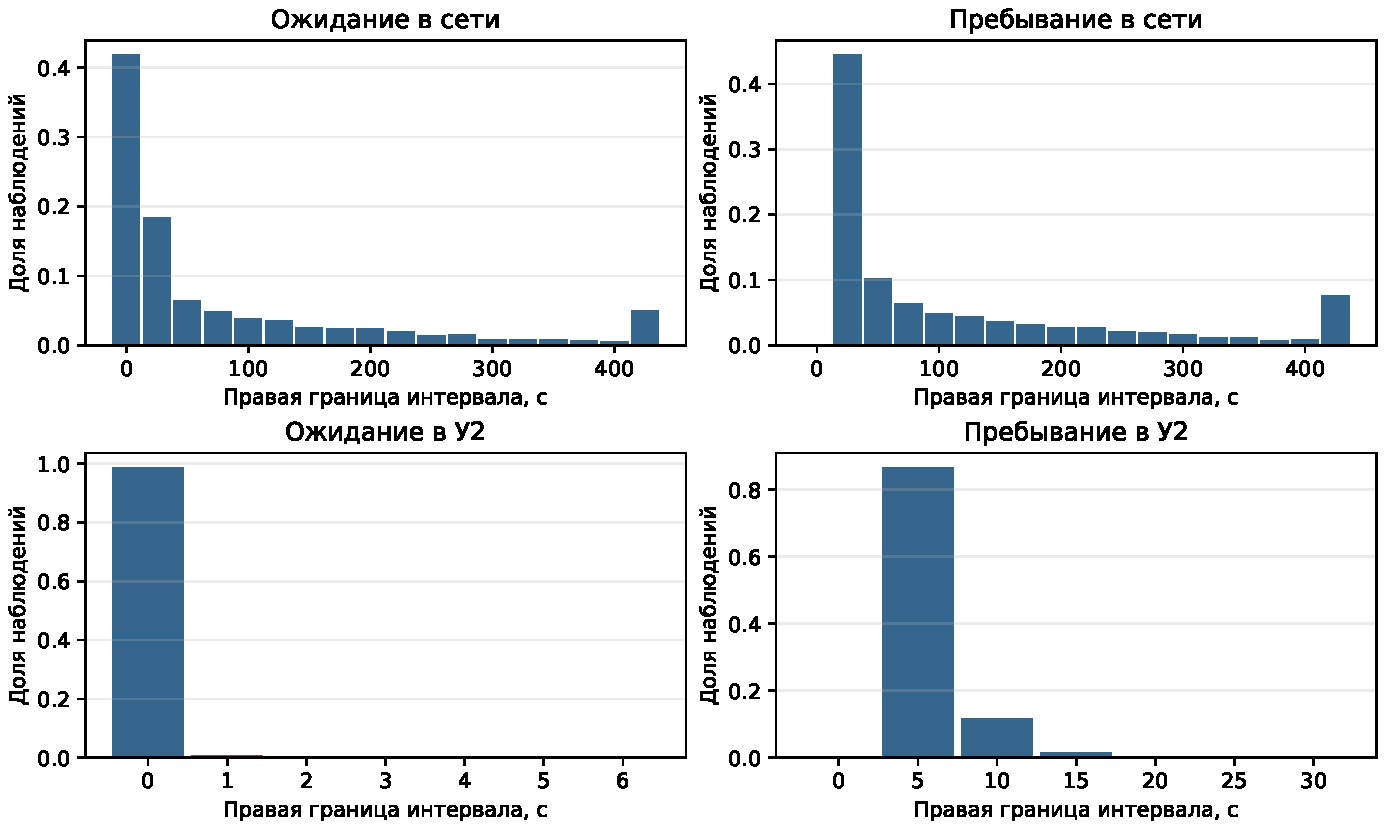
\includegraphics[width=.96\textwidth]{../out/part2/gpss_open_histograms.pdf}
 \caption{Гистограммы из GPSS World для разомкнутой сети с простейшим
 входом и экспоненциальным обслуживанием при заданной \(\rho_3=0{,}90\)}
 \label{fig:p2-open-hist}
\end{figure}

\clearpage
\section{Работа с моделями в GPSS World}
\label{sec:evidence}

\subsection{Двухприборная СМО}

На рисунках~\ref{fig:gp-system-model}–\ref{fig:gp-system-report}
показаны последовательные шаги контрольного опыта системы 33.
После трансляции выполнен прогрев на \(10\,000\) исходов. Затем
команда \texttt{RESET} сбросила статистику, и команда
\texttt{START 120000} запустила измерительный прогон.

\begin{figure}[H]
 \centering
 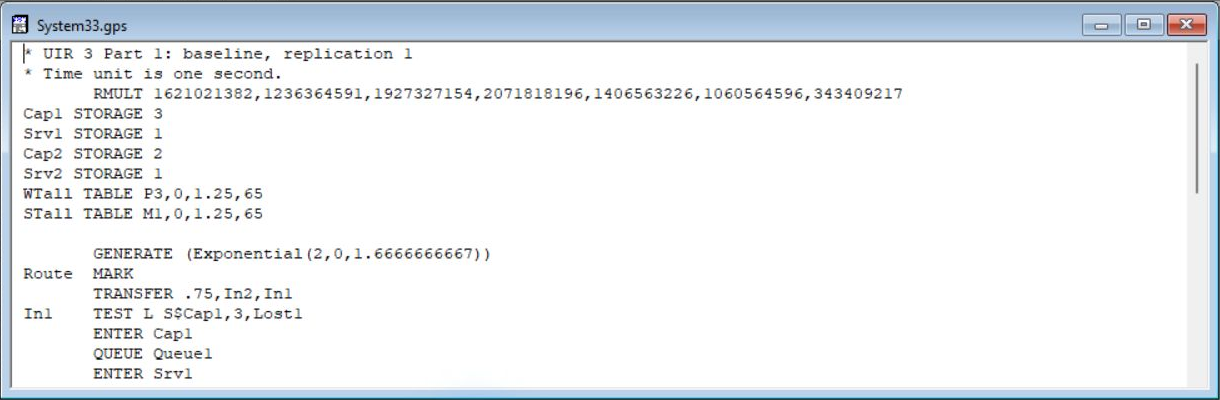
\includegraphics[width=.96\textwidth]{evidence/01_model_system33.png}
 \caption{Исходная модель системы 33 в редакторе GPSS World.
 Первая ветвь вмещает три заявки всего, вторая — две}
 \label{fig:gp-system-model}
\end{figure}

\begin{figure}[H]
 \centering
 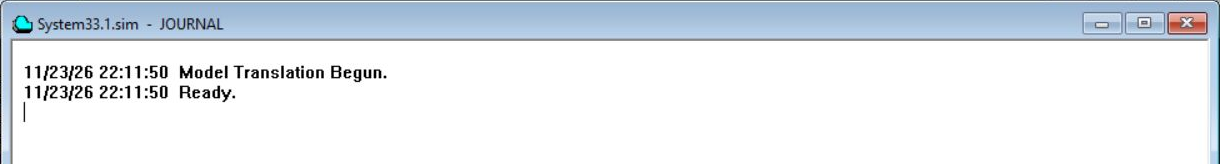
\includegraphics[width=.96\textwidth]{evidence/02_translation_system33.png}
 \caption{Журнал трансляции модели. Сообщение \texttt{Ready} подтверждает
 готовность имитационной модели к запуску}
 \label{fig:gp-system-translation}
\end{figure}

\begin{figure}[H]
 \centering
 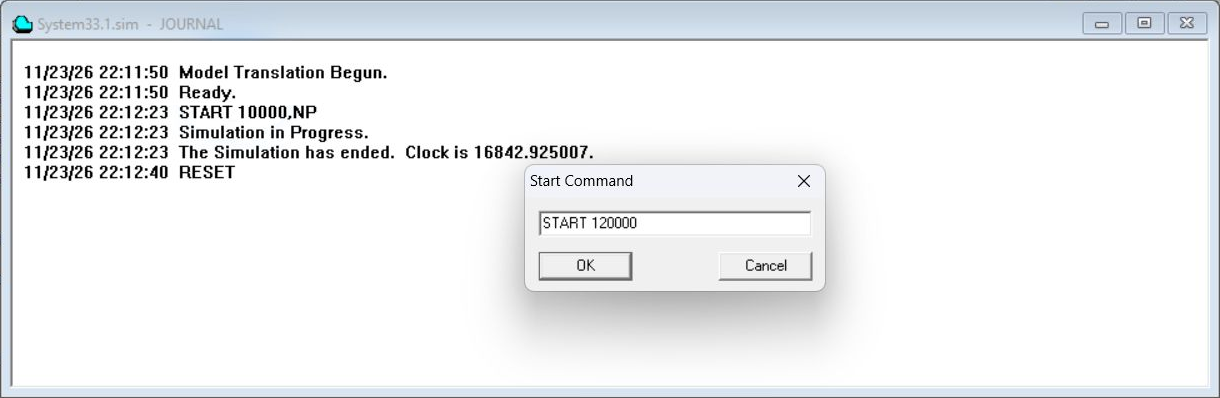
\includegraphics[width=.96\textwidth]{evidence/03_start_system33.png}
 \caption{Настройка измерительного прогона. Журнал показывает выполненный
 прогрев и сброс статистики, в диалоге задана команда \texttt{START 120000}}
 \label{fig:gp-system-start}
\end{figure}

\begin{figure}[H]
 \centering
 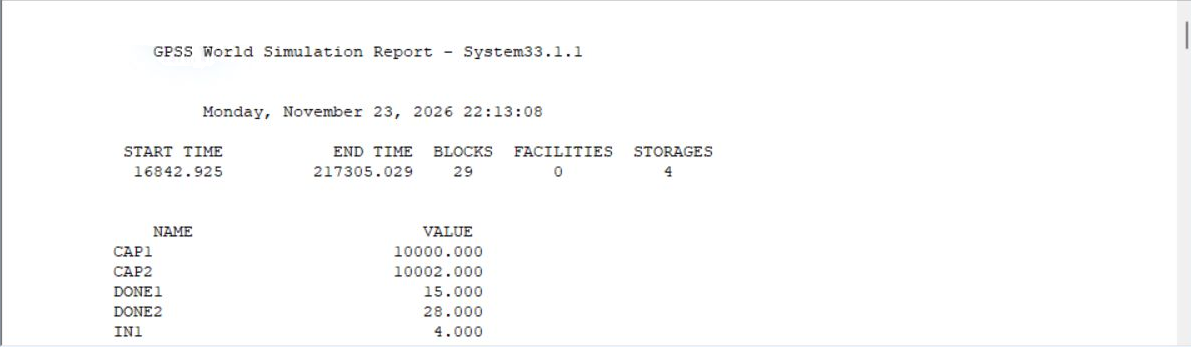
\includegraphics[width=.96\textwidth]{evidence/04_report_system33.png}
 \caption{Стандартный отчёт системы 33. Измерительный интервал
 \(16\,842{,}925\)–\(217\,305{,}029\) с}
 \label{fig:gp-system-report}
\end{figure}

\subsection{Замкнутая сеть M3}

На рисунке~\ref{fig:gp-network-model} открыта контрольная модель
с шестью циркулирующими заявками, а на рисунке~\ref{fig:gp-network-report}
виден отчёт прогона после \(10\,000\) с прогрева.
Статистика собрана за \(200\,000\) с модельного времени.

\begin{figure}[H]
 \centering
 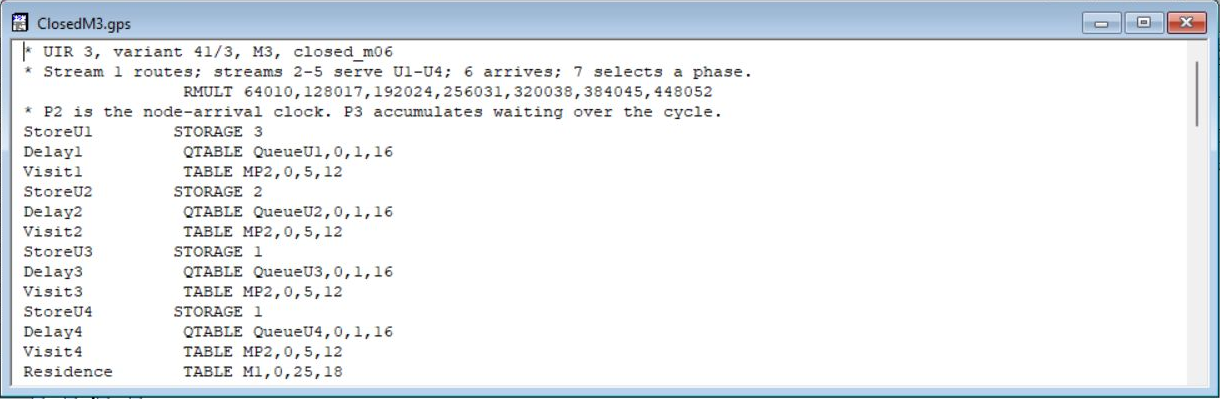
\includegraphics[width=.96\textwidth]{evidence/05_model_network.png}
 \caption{Модель замкнутой сети M3 в редакторе GPSS World.
 Параметры четырёх узлов заданы командами \texttt{STORAGE}}
 \label{fig:gp-network-model}
\end{figure}

\begin{figure}[H]
 \centering
 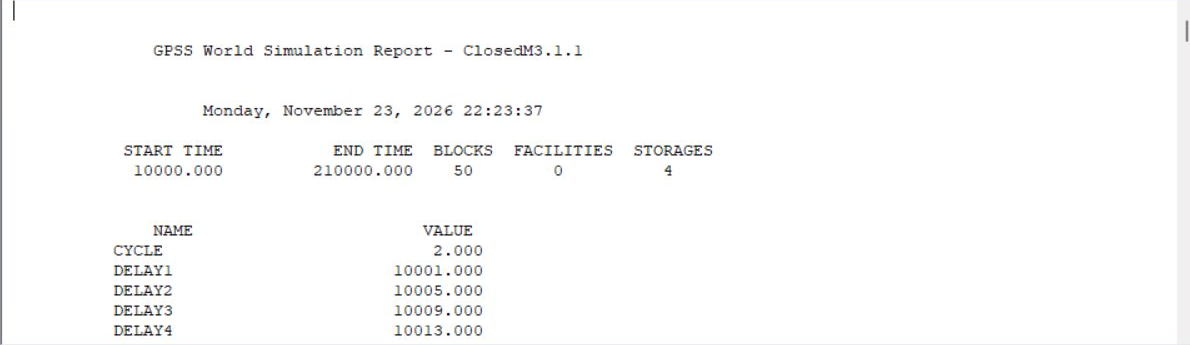
\includegraphics[width=.96\textwidth]{evidence/06_report_network.png}
 \caption{Стандартный отчёт контрольного прогона замкнутой сети при \(M=6\)}
 \label{fig:gp-network-report}
\end{figure}

\clearpage
\subsection{Серия парных прогонов сети M3}

На рисунке~\ref{fig:gp-network-campaign} показан журнал эксперимента,
который сравнивает замкнутую и разомкнутую сети при сопоставимой
интенсивности. Записи с отметками \(100\,000\) и \(900\,000\) с
соответствуют концу прогрева и измерения. Процедура PLUS сохраняет
сводку после каждого измерения в CSV.

\begin{figure}[H]
 \centering
 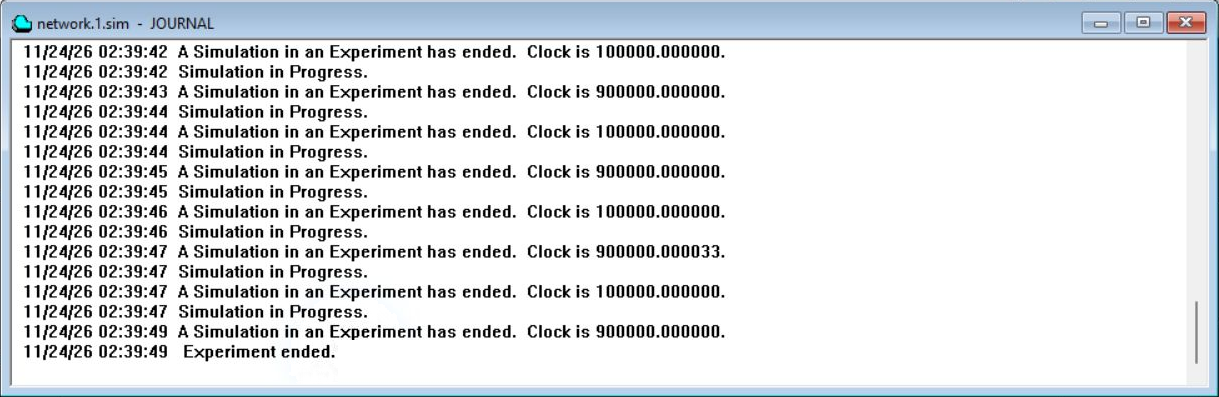
\includegraphics[width=.96\textwidth]{evidence/07_campaign_network.png}
 \caption{Журнал \texttt{network.1.sim} после завершения серии парных прогонов}
 \label{fig:gp-network-campaign}
\end{figure}

\section{Выводы}

Для системы 33 измерения GPSS World согласуются со стационарным
расчётом УИР~2. Максимальное относительное расхождение шести
характеристик составило \(0{,}79\%\). При одном и том же среднем
интервале между заявками наибольшая доля потерь была
у гиперэкспоненциального потока. Дополнительные места в очереди
снижали долю отказов, но увеличивали время ожидания.
Оценка длительности переходного режима
зависит от входного потока, нагрузки и выбранного критерия сходимости.

При исходных параметрах узел У3 ограничивает производительность
сети M3 до \(1/14\) заявки/с. При допуске \(2\%\) к этому пределу
в замкнутой сети нужно как минимум шесть заявок. Когда в У3
сокращали время обслуживания или добавляли приборы, узким местом
становился У1.

При равном потоке и экспоненциальном обслуживании средний цикл
замкнутой сети занял около \(85\) с. В разомкнутой сети с простейшим
входом заявки проводили в системе в среднем около \(1062\) с.
В замкнутой сети фиксированное число заявок ограничивает и длину
очереди. В разомкнутой сети при нагрузке, близкой к предельной,
в У3 может скопиться больше заявок. При такой нагрузке среднее
время в разомкнутой сети сильно менялось от прогона к прогону.
Смена закона обслуживания в У2 сильнее отразилась на временах
ожидания и пребывания в узле, чем на загрузке сети.


\clearpage
\appendix
\section{Листинги моделей GPSS World}

\lstset{language={},basicstyle=\ttfamily\fontsize{7.5}{9}\selectfont,
  columns=fullflexible,keepspaces=true,showstringspaces=false,breaklines=true}
\subsection{Контрольная модель двухприборной СМО}
\lstinputlisting{../models/part1/baseline.gpss}

\subsection{Замкнутая модель сети M3}
\lstinputlisting{../models/part2/closed.gpss}

\subsection{Разомкнутая модель сети M3}
\lstinputlisting{../models/part2/open.gpss}

\end{document}
